\documentclass[10pt]{amsart}
%\usepackage{amsmath}
\usepackage[utf8]{inputenc}
\usepackage{graphicx}
\usepackage{xcolor}
\usepackage[legalpaper, margin=1.5in]{geometry}
\usepackage{fancyvrb}
\usepackage{url}
\usepackage{etoolbox}

% fonts
\input{ArtNouvc.fd}
\newcommand*\initfamily{\usefont{U}{ArtNouvc}{xl}{n}}
\usepackage[T1]{fontenc}
\usepackage{tgbonum} % change font


% from https://www.pinterest.co.uk/pin/88664686405122253/
\definecolor{C1}{RGB}{141, 125, 158} %purple
\definecolor{C2}{RGB}{63,56,47} % yellow
\definecolor{C3}{RGB}{99,151,153} % green
\definecolor{C4}{RGB}{195,106,99} % red
\definecolor{C5}{RGB}{124, 132, 128}
\definecolor{C6}{RGB}{67, 69, 75}

\patchcmd{\section}{\normalfont}{\color{C5}}{}{}
\patchcmd{\subsection}{\normalfont}{\color{C5}}{}{}


\newcommand{\dfn}[1]{\bf  \color{C2}{#1}}
\renewcommand{\FancyVerbFormatLine}[1]{\color{C3}{>\,\,#1}}
    
\newtheorem{thm}{Theorem}

\newtheoremstyle{exercise}
{}                % Space above
{}                % Space below
{\color{C4}\slshape}        % Theorem body font % (default is "\upshape")
{}                % Indent amount
{\bfseries}       % Theorem head font % (default is \mdseries)
{.}               % Punctuation after theorem head % default: no punctuation
{ }               % Space after theorem head
{}                % Theorem head spec
\theoremstyle{exercise}
\newtheorem{exercise}{Exercise}


\newtheoremstyle{example}
{}                % Space above
{}                % Space below
{\color{C1}\slshape}        % Theorem body font % (default is "\upshape")
{}                % Indent amount
{\bfseries}       % Theorem head font % (default is \mdseries)
{.}               % Punctuation after theorem head % default: no punctuation
{ }               % Space after theorem head
{}                % Theorem head spec
\theoremstyle{example}
\newtheorem{example}{Example}

\newtheoremstyle{solution}
{}                % Space above
{}                % Space below
{\color{C5}}        % Theorem body font % (default is "\upshape")
{}                % Indent amount
{\bfseries }       % Theorem head font % (default is \mdseries)
{:}               % Punctuation after theorem head % default: no punctuation
{\newline}               % Space after theorem head
{}                % Theorem head spec
\theoremstyle{solution}
\newtheorem*{solution}{Solution}


\newcommand{\mcS}{\mathcal S}
\newcommand{\mcR}{\mathcal R}
\newcommand{\mcC}{\mathcal C}
\newcommand{\bS}{{\boldsymbol S}}
\newcommand{\bR}{{\boldsymbol R}}
\newcommand{\bC}{{\boldsymbol C}}
\newcommand{\ba}{{\boldsymbol a}}
\newcommand{\bb}{{\boldsymbol b}}
\newcommand{\bs}{{\boldsymbol s}}
\newcommand{\bff}{{\boldsymbol f}}
\newcommand{\br}{{\boldsymbol r}}
\newcommand{\bx}{{\boldsymbol x}}
\newcommand{\bt}{{\boldsymbol t}}
\newcommand{\bv}{{\boldsymbol v}}
\newcommand{\bu}{{\boldsymbol u}}
\newcommand{\bw}{{\boldsymbol w}}
\newcommand{\bc}{{\boldsymbol c}}
\newcommand{\be}{{\boldsymbol e}}
\newcommand{\bq}{{\boldsymbol q}}
\newcommand{\bphi}{{\boldsymbol \phi}}
\newcommand{\brho}{{\boldsymbol \rho}}
\newcommand{\btau}{{\boldsymbol \tau}}
\newcommand{\reals}{\mathbb R}
\newcommand{\ints}{\mathbb N}
\newcommand{\E}{\mathbb E}
\newcommand{\Prob}{\mathbb P}

\title{\Huge \color{C1} Statistical models and simulation}
\author{\color{C1} Ethan Levien}
\date{April 2022}

\begin{document}

\maketitle

\tableofcontents



\section{Statistical models}
A central concept to this course is that of a {\dfn model}. Before doing any mathematics, let's reflect on the notion of a model in the abstract.

\begin{exercise}
What does it mean to model something?
\end{exercise}




Broadly speaking, models are simplified representations of the world\footnote{Model is sometimes used interchangeably with {\dfn theory}, although I usually think of models as being smaller in scope.} There are many ways to represent models, but in science (and life), we often use {\dfn mathematical models}.
For example, you might be familiar with Newton's equation:
\begin{equation}\label{eq:fma}
F = ma
\end{equation}
which related the force ($F$) acceleration ($a$) and mass ($m$) of a particle. This a mathematical model of the motion of a  (non-relativistic) particle in a force field. While it isn't always true, it holds for such a wide range of applications that we call it a \emph{fundamental} law of nature, and it turns out to be extremely powerful. We can combine Newton's equation with other fundamental lows build models of more complicated systems involving many particles. For example, to build a model of planetary motion, we can combine Newton's equation with his other law of gravity, which states that the gravitation force between two objects of masses $m_1$ and $m_2$ a distance $r$ from each other is
\begin{equation}
F = G\frac{m_1m_2}{r^2}
\end{equation}
where $G$ is a constant.
We refer to these types of models -- that is, those which are built upon fundamental laws of nature -- as {\bf mechanistic} models.
%Other mechanistic models are the equation of the number of chemicals in a well-mixed vessel (based on the law of mass action) and the equation for the

In statistics, we are often interested in problems where nothing remotely close to a fundamental laws exist. Instead, they are based directly on observations (data) or our intuitions. In economics, for example, models are built in numerous assumptions about the human nature, many of which may seem obvious or intuitive. However, our intuition about economics is itself shaped by the particular economic system we experience, and in reality these assumptions regularly break down as economic conditions change.  We will call these {\dfn phenomenological models}. Such models still be quite useful provided we are aware of their limitations. Of course, there is not sharp distinction between mechanistic and phenomenological models, but the distinction is helpful nonetheless.


Often our models cannot make exact predictions about the value of a variable (this is true in both mechanistic and phenomenological models, but especially the latter). Instead, they only tell us the probability that a variable has a certain value, or falls within a range of values. For example, if we were to construct a model of the $(y)$ of all the pine trees in New Hampshire as a function of their age $(x)$, we might begin by searching for a function $f$ such that
\begin{equation}
y = f(x)
\end{equation}
However, if we take a {\dfn sample} of the population, meaning we go out and measure the height of some trees for which we know the age, we will quickly find that trees of the same age can have different heights.   This variation will be as result of many variables which are not in our model, e.g. the surrounding, the specific subspecies of pine, genetic variation within a subspecies to name just a few. We could construct a more sophisticated model which includes, say, the DNA sequence of the tree ($g$):
\begin{equation}
y = f(x,g).
\end{equation}
This model would presumably have less variation. That is, if we collect a sample of trees for which we know the height and DNA sequence, we would find that the variation between trees with the same DNA and height is less than the variation between trees with only the same height. Yet variation will remain unless we include all the variables which effect tree height. This is of course impossible, as there are million, perhaps billions of such variables and their effects are far beyond our understanding of biology. Moreover, it is not so useful to include these variables, since we can actually measure most of them and many of them will have small effects. One approach to dealing with these ``hidden" sources of variation is to define a {\dfn statistical model}, where $y$ is not the same for each tree of the same height, but is instead a {\dfn random variable}. On type of a statistical model is a regression model
\begin{equation}\label{eq:reg}
y = f(x) + \epsilon
\end{equation}
where $\epsilon$ is a random variable (usually one that is zero, on average).

%\begin{exercise}
%When we write down a model, statistical or otherwise, we make assumptions. What are some of the assumptions we have made by writing down Equation \eqref{eq:reg}? Hint: think about other ways in which you might compute a random term, $\epsilon$, with a function like $f$.
%\end{exercise}


\section{Random variables and distributions}

The rigorous mathematical theory for random variables is very useful, but requires certain machinery which is beyond the scope of these notes. Fortunately, we go a long way without such formalism. For our purposes, a random variable can be understood as a variable which we cannot predict prior to an observation, regardless of how much information we have.
We can define the space of  {\dfn outcomes} as all the possible values that a random variable may take on. The outcomes for the roll of a dice are $1,2,\dots,6$ for the dice, or positive numbers for the height of a tree.  Usually the outcomes are numbers, even if we use a number to represent a non-numerical quantity (e.g. someone's gender). In probability theory, one distinguishes between outcomes and {\dfn events} -- the latter are subsets of outcomes. For example, we might refer to the event that the roll of a die is grater than $2$. It's good to be aware of these definitions, but you don't need to memorize them.



We can describe a characterize a random variable using  a {\dfn probability distribution}, which maps a set of possible events to real numbers between 0 and 1.  For example, suppose we ask a random student in the college whether they were born in the US. A probability distribution $P(Y)$ which \emph{models} their answer is the {\dfn Bernoulli distribution},
\begin{equation}
P(Y) = \left\{ \begin{array}{cc}
q & Y={\rm YES}\\
1-q & Y={\rm NO}
\end{array}
 \right.
\end{equation}
where $q$ is the fraction of students in the college who were born in the US. We say that $q$ is a {\dfn parameter} in our model because regardless of it's value our model is still a Bernoulli distribution.
 It is very important that the sum of $P(Y)$ over all possible outcomes is $1$ -- this is simply saying that we are certain one of the outcomes will happen.

 The Bernoulli distribution is our default model for any variable that can take two possible outcomes, usually abstracted as $0$ or $1$.  In order to state that a Bernoulli distribution is a model for some random variable $Y$, we write
\begin{equation}
Y \sim {\rm Bernoulli}(q).
\end{equation}
We might also say ``$Y$ \emph{follows} as Bernoulli distribution" or ``$Y$ is a Bernoulli random variable".
More generally, we say that a variable in a model follows a given distribution by writing
\begin{equation}
{\rm Variable} \sim {\rm Distribution}({\rm parameters}).
\end{equation}
We will sometimes use $\theta$ to denote the parameters. 


Turning back to the example of our survey, let's suppose we don't have information about every students in the college. Rather, a survey of five students from this class is conducted, finding $4$ yeses and $1$ no. It seems like our best estimate of $q$ should be the fraction of $4/5$. This is an example of {\dfn statistical inference}. More generally, we use statistical inference to make predictions about things we don't observe based one what we do observe (data).





%\begin{exercise}
%Suppose we are counting the number  $\{1,2,3,4,5,6,7,8,9,12\}$
%\end{exercise}
\section{Python as a tool for statistical modeling}
When we generate samples using a computer we call them {\dfn simulations}. We will use python to perform simulations, and it is therefore important to have a basic understanding of the python language. It is assumed that you will go through the separate python tutorial notebook. For convenience, here is a very brief summary of some things you will need to do in Python. 
First, we will assign variables and perform arithmetic. These operations are pretty intuitive: 
\begin{Verbatim}
x = 1
y = 2
z = x + y
print(z)
z = x*y 
print(z)
\end{Verbatim}
We will work heavily with vectors, or lists of numbers in this course. 
\begin{Verbatim}
a = [1,2,3] # make empty list
a.append(5) # add 5 to the end of the list
print(a) # print the list
print(a[2])	# index the list
print(a[0:2])	
print(a[a>2]) # obtain a subset of the list
# easy way to make an array
a = range(5)
print(a[0])
\end{Verbatim}
We will work with a package called numpy, which provides a wrapper for the python list affording us some additional functionality. 
\begin{Verbatim}
import numpy as np # import the numpy package
a = np.zeros(5)
a = np.array([0,0,0,0,0])
# advantage of numpy arrays:
a = np.array([1,2,3])
b = np.array([5,3,2])
a + b
# get the length of an array 
len(a)
# generate array 
a = np.linspace(0,1,100)
print(a)
\end{Verbatim}
Loops allow us to repeat an operation, or carry out an operation over some range of values
\begin{Verbatim}
for k in range(5):
	print(k)	
\end{Verbatim}
The same thing can be achieved with a while loop 
\begin{Verbatim}
k = 0
while k<5: 
	print(k)
	k = k+1
\end{Verbatim}

In many instances, it is helpful to put code we will reuse in a function. 
\begin{Verbatim}
def test_func(z)
	k = 0
	while k<z: 
		print(k)
		k = k+1
 	return k
a = test_func(k)
\end{Verbatim}


\begin{exercise}
Consider the following code: 
\begin{Verbatim}
for i in range(5):
  for j in range(i)
    print(i)
    print(",")
  println()
\end{Verbatim}
Based on the output of this code, what do you think \verb|println()| does? Check the documentation to confirm you answer. Check the documentation to confirm your answer. 
Then, modify this code and put it in a function \verb|print_triangle(n)| which prints 
\begin{Verbatim}
1,1
1,2,2
1,2,3,3
.
.
.
1,2,3,...,n,n
\end{Verbatim}
\end{exercise}
\begin{solution}
Making only a few changes to the existing code and putting it in a function 
\begin{Verbatim}
def print_triangle(n)
    for i in range(n):
      for j in range(i)
        print(i)
        print(",")
      print(i)
      println()
\end{Verbatim}
\end{solution}
%\begin{exercise}
%Determine what the following lines for code will output
%\begin{enumerate}
%\item What will be the value of $z$ after the following line of code is run?
%\begin{Verbatim}
%z = 1
%for k in range(3):
%  z = z+k
%\end{Verbatim}
%\item What will the following code print?
%\begin{Verbatim}
%x = 11
%k = 1
%while x>2:
%  x = x-2
%  print(k)
%  k = k+1
%\end{Verbatim}
%
%\item Consider the code
%\begin{Verbatim}
%for i in range(5):
%  for j in range(i)
%    print(i)
%    print(",")
%  println()
%\end{Verbatim}
%modify this code to print
%\begin{Verbatim}
%1 *
%1,2 *
%1,2,3 *
%1,2,3,4 *
%\end{Verbatim}
%\end{enumerate}
%\end{exercise}


\subsection{Simulations}
 Here, we will focus on tools relevant for statistics. In Python, we can simulate random variables using the \verb|numpy| library:
\begin{Verbatim}
import numpy as np
q = 0.5
y = np.random.choice(range(2),p=[q,1-q])
 \end{Verbatim}
 We can generate multiple samples using a for loop
\begin{Verbatim}
n_samples = 100
y = np.zeros(n_samples) # makes an empty list (i.e. array) of n_samples zeros.
for k in np.range(n_samples):
  y[k] = np.random.choice(range(2),p=[q,1-q])
 \end{Verbatim}
A simpler way of doing this is
\begin{Verbatim}
y = np.random.choice(range(2),n_samples,p=[q,1-q])
 \end{Verbatim}


  The more general form of this command is
\begin{Verbatim}
y = np.random.choice(range(k),n_samples,p=[q_1,q_2,...,q_k])
 \end{Verbatim}
 where $q_1 + \cdots q_k = 1$. This will generate a sample from



 \begin{exercise}
Write down the probability distribution for a the value rolled by a 6 sided die and use the random choice function in python generate simulated rolls of your dice. Then, write down a probability distribution for a $6$ sided die with the one face replaced with a two.
\end{exercise}
\begin{solution}
For the fair die we have
\begin{Verbatim}
y = np.random.choice(range(6),n_samples,p=[1/6,1/6,1/6,1/6,1/6,1/6])
\end{Verbatim}
For the other one we have
\begin{Verbatim}
y = np.random.choice(range(6),n_samples,p=[0,2/6,1/6,1/6,1/6,1/6])
\end{Verbatim}
\end{solution}

 We can also generate simulations of more complex random variables using simple ones. For, example:
 \begin{example}
Write a function which simulates flipping a fair coin until we get $2$ heads in a row.
\end{example}
\begin{solution}
\,
\begin{Verbatim}
def flip_until_two():
  num_heads = 0
  total_flips = 0
  while num_heads <2:
    y = np.random.choice([0,1])
    if y == 0:
      num_heads = 0
    else:
      num_heads = num_heads + 1
    total_flips = total_flips + 1
  return total_flips
 \end{Verbatim}
 \end{solution}



\begin{exercise}
By changing the code above, write a function that rolls a dice until we get two ones in a row.
\end{exercise}
\begin{solution}
We need to change (1) the distribution we sample $y$ from and (2) the condition to stop. 
\begin{Verbatim}
def dice_until_two():
  num_ones = 0
  total_rolls = 0
  while num_ones <2:
    y = np.random.choice([1,2,3,4,5,6])
    if y == 0:
      num_ones = 0
    else:
      num_ones = num_ones + 1
    total_rolls = total_rolls + 1
  return total_rolls
 \end{Verbatim}
\end{solution}

\subsection{Visualization}

 An important tool for visualizing samples is a histogram
\begin{Verbatim}
plt.hist(samples,100,density=true)
 \end{Verbatim}
 The histogram shows us the frequency of different outcomes.



\subsection{Monte Carlo}
Often, we run many simulations of a model in order to say something about the distribution without performing any analytical calculations. We call these {\dfn Monte Carlo} simulations.
\begin{example}
Suppose we flip a coin until we get $2$ heads in a row, as we implemented above, and let $J$ denote the number of flips. Use Monte Carlo simulations the chance that $J>5$. Also plot a histogram. 
\end{example}
\begin{solution}
We will make a loop which performs the coin flipping many times and save the number of flips. 
\begin{Verbatim}
n_monte = 1000
Js = np.zeros(n_monte)
for k in range(n_monte):
  Js[k] = flip_until_two()
len(Js[Js>5])/len(Js)
plt.hist(Js)
 \end{Verbatim}
\end{solution}







\subsection{Means and variances}
There are ways in which we summarize attributes of random variables.
If we have many samples $Y_1,Y_2,\dots,Y_n$ of a random variable (e.g. answers to a survey question), the {\dfn sample mean} is defined as
\begin{equation}
\bar{y} = \frac{1}{n}\sum_{i}y_i
\end{equation}
 Often it is useful to quantify the deviations from the mean. Suppose $y_i$ can take on outcomes $y_1,\dots,y_m$. If $n$ is large, then the fraction of samples for which $Y_1= y_1$ will be $P(Y_1=y_1)$.
 \begin{equation}
\bar{y} \approx \frac{1}{n} \sum_{\rm outcomes} y_in_i= \sum y_i P(Y_i=y_i)
\end{equation}
The expression on the right is the definition of expected value, often denoted $\E[Y]$.



 For this, we have the {\dfn sample standard deviation}
\begin{equation}
\sigma = \sqrt{\frac{1}{n-1}\sum_{i}(y_i-\bar{y})^2}.
\end{equation}
We will see why this makes sense as a measure of how spread our a distribution is later on when we talk about inference. For large $n$, this converges to the square root of the variance
\begin{equation}
{\rm Var}(Y) = \sum (y_i - \E[Y])^2 P(Y_i=y_i).
\end{equation}



Importantly, we can always calculate the mean and standard deviation of a sample, regardless of the distribution it has been drawn from. However, we need to be careful, as the results may not be so meaningful.


%\begin{example}
%Write a python function in python that computes the mean and standard deviation
%\end{example}


In python, functions for implementing the mean and standard deviation are follows:
\begin{Verbatim}
np.mean(y)
np.std(y)
\end{Verbatim}

%\begin{example} Use Monte Carlo simulations to study how the mean and variance of the number of flips it takes to get two
%
%\end{example}


\begin{example}
Verify that the formula for the mean and standard deviations with Monte Carlo simulations
\begin{align}\label{eq:bern_sts}
\E[Y] = q
\end{align}
\end{example}

\begin{solution}
The following code will estimate the mean and standard deviations for various values of $q$:
\begin{Verbatim}
def mean_bern(q):
  sample = np.random.choice([0,1],500,p=[1-q,q])
  return np.mean(sample)

# generates one hundred evenly spaced numbers between 0 and 1
q_range = np.linspace(0,1,100)
means = np.zeros(len(q_range))
for j in range(len(q_range)):
  means[j]= mean_std_bern(q_range[j])
\end{Verbatim}
Here is a plot of the mean compared to the prediction
\begin{Verbatim}
fig,ax = plt.subplots(figsize=(5,2))
ax.plot(q_range,means)
ax.plot(q_range,q_range,"k--")
\end{Verbatim}

\end{solution}


\begin{exercise}
Modify the code above to verify that
\begin{equation}
 \sqrt{{\rm Var}(Y)} = \sqrt{q(1-q)}
\end{equation}
\end{exercise}
\begin{solution}
We only need to change the mean to the standard deviation
\begin{Verbatim}
def std_bern(q):
  sample = np.random.choice([0,1],500,p=[1-q,q])
  return np.std(sample)

# generates one hundred evenly spaced numbers between 0 and 1
q_range = np.linspace(0,1,100)
means = np.zeros(len(q_range))
for j in range(len(q_range)):
  stds[j]= std_bern(q_range[j])
\end{Verbatim}
\end{solution}










\section{Joint probabilities, Independence} We introduce, very briefly, the concepts of independence and conditioning. Just as we have considered single random variables, we can consider multiple random variables within the same model. Suppose we have two Bernoulli random variables $Y_1$ and $Y_2$ which model whether a person has mutations at two different genomes.  In this case, we need a model of both variables together:
\begin{equation}
\Prob(Y_1,Y_2) = \left\{ \begin{array}{cc}
q_{00} & \text{ if }Y_1=0 \text{ and } Y_2 = 0\\
q_{01} & \text{ if }Y_1=0 \text{ and } Y_2 = 1\\
q_{10} & \text{ if }Y_1=1 \text{ and } Y_2 = 0\\
q_{11} & \text{ if }Y_1=1 \text{ and } Y_2 = 1\\
\end{array}
 \right.
\end{equation}


\begin{example}
Write python code to generate a sample of $Y_1$ and $Y_2$ using
\begin{equation}
q_{00} = 1/8,\quad q_{01} = 1/8,\quad q_{10} = 1/4, \quad q_{11} = 1/2
\end{equation}
\end{example}
\begin{solution}
There are $4$ outcomes, so we can identify each with a number as follows:
\begin{equation}
(0,0) \to 1,\quad (0,1) \to 2,\quad (1,0) \to 3,\quad (1,1) \to 4
\end{equation}
We then use the random choice function
\begin{Verbatim}
np.random.choice([1,2,3,4],p=[1/8,1/8,1/4,1/2])
\end{Verbatim}
\end{solution}



The probability distribution $P(Y_1,Y_2)$ tells us the probabilities for observing \emph{both} variables together, e.g. observing a person with both mutations. It does not directly tell us the probabilities of observing e.g. someone with only one mutation. This can be obtained via marginalization; that is, summing over the other variable:
\begin{equation}
P(Y_1)  = \sum_{y}P(Y_1,y) = P(Y_1,0)  +P(Y_1,1)
\end{equation}
where in the general the sum is taken over all possible outcomes for the second variable. $\Prob(Y_1)$ is defined similarly. Sometimes, we are interested in the value of a random variable given, or {\dfn conditioned on} another random variable. The probability of that $Y_1 = 1$ if we know $Y_2 = 0$, denoted $P(Y_1=1|Y_2=0)$ would be the chance that gene 1 has a mutation in a person if we know there is no mutation at gene 2. Said another way, we are looking at the chance of someone having a mutation at gene 1 among only those people that do not have a mutation at a gene 2. 


How do we calculate this? Bayes theorem tell us that for two random variables $X$ and $Y$
\begin{equation}\label{eq:bayes}
\Prob(Y|X) = \frac{P(Y,X)}{P(X)}
\end{equation}
Two variables are said to be {\dfn independent} if $\Prob(Y|X)  = P(X)$. This is also true for events. For our purposes, it is more important to understand the process of conditioning with data. 

\begin{example}
Consider the data $\{1,2,2,1,3,4\}$ where each number corresponds to a different configuration of the two genes. Estimate $P(Y_1=0|Y_2=0)$ from Monte Carlo simulations
\end{example}
\begin{solution} 
First we generate some data
\begin{Verbatim}
y = np.random.choice([1,2,3,4],p=[1/8,1/8,1/4,1/2])
\end{Verbatim}
We can then obtain the sample conditioned on $Y_2$ having the mutation: 
\begin{Verbatim}
y[y ==1 or y==3]
\end{Verbatim}
The conditional probability would be 
\begin{Verbatim}
len(y_sub[y==1])/len(y_sub)
\end{Verbatim}
\end{solution}




%
%\begin{example}
%In this case, we have
%\begin{equation}\label{eq:ex_bayes}
% \frac{P(Y_1=2,X_2=0)}{P(Y_2=0)} = \frac{q_{10}}{q_{10}+q_{01}}
%\end{equation}
%Use Monte Carlo simulations to confirm Equation  \eqref{eq:ex_bayes} for the values given in exercise ??.
%\end{example}
%
%\begin{solution}
%This is achieved by the following code:
%\begin{Verbatim}
%y = np.random.choice([1,2,3,4],1000,p=[1/8,1/8,1/4,1/2])
%y_sub = y[y ==1 or y==3]
%len(y_sub[y==1])/len(y_sub)
%\end{Verbatim}
%\end{solution}

\begin{exercise}
Let $Y$ be the value of a 6 sided die, but the one face has been replaced with a two (so there are two, two faces). What is $\Prob(Y=3|Y>2)$? Confirm you answer with Monte Carlo simulations.
\end{exercise}

\begin{solution}
This is achieved by the following code:
\begin{Verbatim}
y = np.random.choice([1,2,3,4,5,6],1000,p=[1/6,1/6,1/6,1/6,1/6,1/6])
y_sub = y[y >2]
len(y_sub[y==3])/len(y_sub)
\end{Verbatim}
\end{solution}




%\begin{exercise}
%In this model you will combine what you've learned to build a model for student birthdays.
%\begin{enumerate}
%\item Construct a model for a statistical model for a students birthday. That is, you should treat a students birthday $Y$ (a number between $1$ and $366$ (to account for leap years).
%\item Write python code which generates samples from this model.
%\item Use Monte Carlo simulations to determine the chance that two students share the same birthday.
%\end{enumerate}
%\end{exercise}





\section{More random variables}

 \subsection{Binomial: Distribution}
A situation that often arrises is that we take many, say $n$, independent samples from a Bernoulli distribution. Now let $Y$ be the number of $1$s. Then $Y$ follows {\dfn binomial distribution}:
\begin{equation}
Y \sim {\rm Binomial}(n,q)
\end{equation}
The binomial distribution has two parameters, $k$ and $p$, and the probability distribution is
\begin{equation}
\Prob(Y) = {n \choose Y}q^{Y}(1-q)^{n-Y}
\end{equation}
The binomial distribution has a mean $qn$ and variance $nq(1-q)$.
We can draw samples from a binomial distribution
 \begin{Verbatim}
y = np.random.binomial(n,p,n_samples)
 \end{Verbatim}


\begin{exercise}
Run simulations of the Binomial distribution and plot the average and standard deviation of the average as a function of $n$. Also plot a few histogram for different $n$. 
\end{exercise}
\begin{solution}
The following code will estimate the mean and standard deviations for various values of $q$:
\begin{Verbatim}
def mean_std_bern(n,q):
  sample = np.random.binomial(n,q,100)
  return np.mean(sample),np.std(sample)

# generates one hundred evenly spaced numbers between 0 and 1
q_range = np.linspace(0,1,100)
means = np.zeros(len(q_range))
stds = np.zeros(len(q_range))
for j in range(len(q_range)):
  means[j],stds[j] = mean_std_bern(q_range[j])
\end{Verbatim}
Here is a plot of the mean compared to the prediction
\begin{Verbatim}
fig,ax = plt.subplots(figsize=(5,2))
ax.plot(q_range,means)
ax.plot(q_range,q_range,"k--")
\end{Verbatim}
and the standard deviations
\begin{Verbatim}
fig,ax = plt.subplots(figsize=(5,2))
ax.plot(q_range,stds)
ax.plot(q_range,np.sqrt((1-q_range)*q_range),"k--")
\end{Verbatim}
\end{solution}


\subsection{Normal distribution and the central limit theorem}

In the previous example, we say that if we take the average of many Bernoulli random variables, we get a histogram that looks a lot like a ``bell curve" with a standard deviation that scales as $1/\sqrt{n}$.

It turns out this is true when we add up \emph{any} random variables which are sufficiently independent (we will make this precise soon). Since the ``bell curve" arrises in the limit where we sum or average many random variables. This motivates us to define the Normal distribution. Unlike previous random variables we've seen, a normal random variable
\begin{equation}
Y \sim {\rm Normal}(\mu,\sigma)
\end{equation}
can take on any number, positive or negative, decimal or integer.
We can generate Normal random variables in python with
\begin{Verbatim}
np.random.normal(0,1)
\end{Verbatim}


We want to describe this random variable in terms of a probability distribution, but the probability for $Y$ to equal any given value of $Y$ is zero. To see this, note that the probabilities must sum to one  In this case, we can describe the probability distribution
\begin{equation}
\Prob(y_1<Y<y_2) = \int_{y_1}^{y_2}f(y)dy
\end{equation}
for a function $f$ called the probability density. It is given by
\begin{equation}
f(y) = \frac{1}{\sqrt{2\pi \sigma}}^{-\frac{-(y-\mu)^2}{2\sigma}}.
\end{equation}

\begin{figure}[h]
\centering
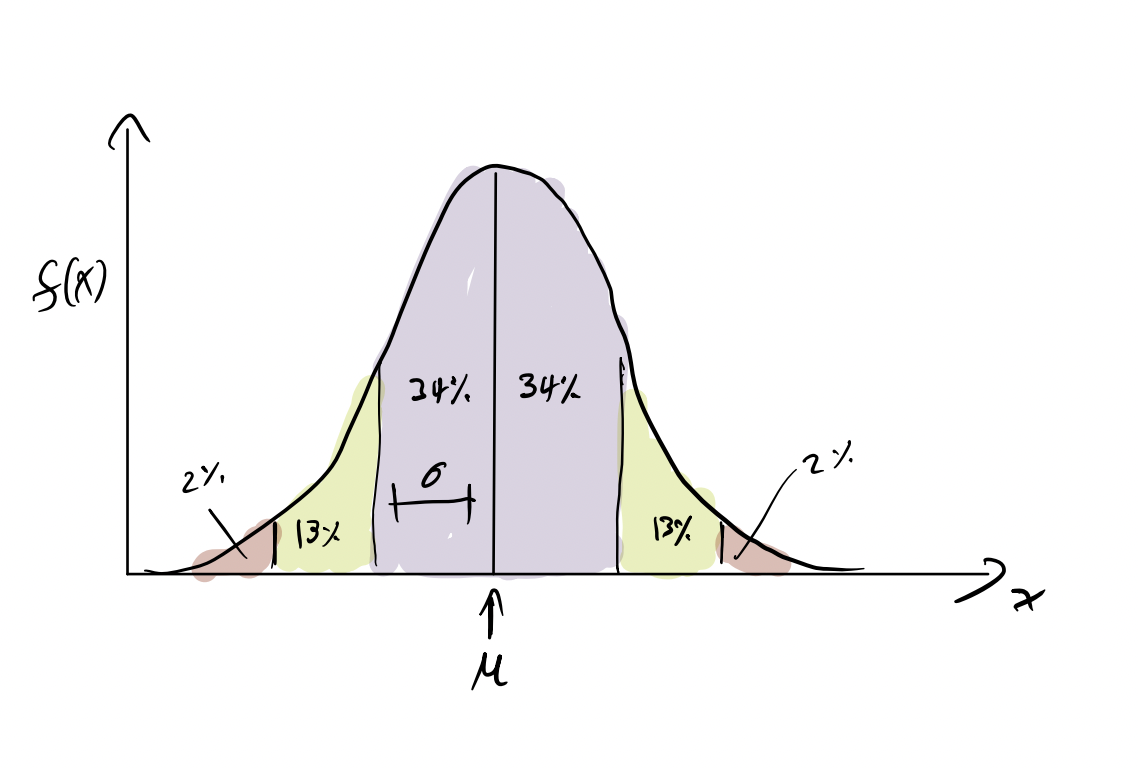
\includegraphics[width=0.8\textwidth]{bellcurve}
\caption{Probabilities in the Normal distribution}
\end{figure}


\begin{example}
Suppose that 
\begin{equation}
Y \sim {\rm Normal}(5,2)
\end{equation}
what is $P(Y>7)$?  Confirm the answer with simulations. 
\end{example}


\begin{exercise}
Suppose that 
\begin{equation}
Z \sim {\rm Normal}(0,1).
\end{equation}
In this case we say that $Z$ is a {\dfn standard normal} random variable. What is the chance that 
\begin{equation}
P(5Y-2>3)
\end{equation}
and confirm you answer with simulations 
\end{exercise}


Going forward, you will need to know the following properties of Normally distributed random variables. Let
\begin{equation}
Y_1 \sim {\rm Normal}(0,1),\quad Y_2 \sim {\rm Normal}(0,1)
\end{equation}
 Then
\begin{align}
aY_1 + b &\sim {\rm Normal}(b,a)\\
aY_1 + bY_2 &\sim {\rm Normal}(0,\sqrt{a^2 + b^2})
\end{align}

%\begin{example}
%Show that if
%\begin{equation}
%Y_1 \sim {\rm Normal}(\mu_1,\sigma_1),\quad Y_2 \sim {\rm Normal}(\mu_2,\sigma_2)
%\end{equation}
%then
%\begin{equation}
%aY_1 + bY_2 + c \sim {\rm Normal}(\mu_1+\mu_2 + c,\sqrt{(a\sigma_1)^2 + (b\sigma_2)^2})
%\end{equation}
%\end{example}

We now return to the connection to sums of random variables and the Binomial distribution. The {\dfn central limit theorem} tells us that for a set of random variables $x_1,\dots,x_n$ with each have $\E[x_i] = \mu_x$ and ${\rm var}(x_i) = \sigma_x^2$,
\begin{equation}
Y = \sum x_i
\end{equation}
is approximately Normal with mean $\mu$ and variance $\sigma/\sqrt{n}$.
In other words Normal random variables emerge when we add up many small sources of randomness.



 \begin{exercise} Another important distribution is the Beta distribution. A random variable 
 \begin{equation}
 Y \sim {\rm Beta}(\alpha,\beta)
 \end{equation}
is characterized by two parameters, $\alpha$ and $\beta$.  
 \begin{Verbatim}
 np.random.beta(1,2,100)
 \end{Verbatim} 
 Experiment with the beta distribution and determine how the two arguments influence the shape of the distribution by plotting histograms. To help guide you, consider exploring the questions 
 \begin{enumerate}
 \item What happens if $\alpha = \beta$? How does $\alpha$ change the shape? 
 \item What happens if $\alpha + \beta =c$ is a constant. 
 \end{enumerate}
\end{exercise}











\end{document}
